\documentclass[aspectratio=169,10pt]{beamer}
\usepackage[utf8]{inputenc}
\usepackage[T1]{fontenc}
\usepackage{lmodern}
\hyphenpenalty=10000
\exhyphenpenalty=10000
\usepackage{booktabs,graphicx,amsmath}
\definecolor{navy}{HTML}{142B43}
\definecolor{teal}{HTML}{007F83}
\definecolor{orange}{HTML}{B55A21}
\definecolor{muted}{HTML}{526273}
\setbeamercolor{normal text}{fg=navy,bg=white}
\setbeamercolor{frametitle}{fg=navy}
\setbeamercolor{structure}{fg=teal}
\setbeamercolor{alerted text}{fg=orange}
\setbeamercolor{block title}{fg=teal,bg=white}
\setbeamercolor{block body}{fg=navy,bg=white}
\setbeamertemplate{navigation symbols}{}
\setbeamertemplate{frametitle}{\vspace{0.15cm}\insertframetitle\par\vspace{0.03cm}{\color{teal}\rule{\textwidth}{0.6pt}}}
\setbeamersize{text margin left=0.6cm,text margin right=0.6cm}
\setbeamerfont{frametitle}{size=\Large,series=\bfseries}
\setbeamerfont{footline}{size=\tiny}
\setbeamertemplate{footline}{\hspace{0.6cm}\color{muted}EAD6034 | Renan de Luca Avila | 28/09/2026\hfill\insertframenumber/\inserttotalframenumber\hspace{0.6cm}\vspace{0.15cm}}
\hypersetup{colorlinks=true,urlcolor=teal,linkcolor=teal,pdftitle={EAD6034 | Previsibilidade e volatilidade do WIN},pdfauthor={Renan de Luca Avila}}
\newcommand{\source}[2]{\par\vfill{\raggedright\tiny\color{muted}#1\quad\href{#2}{Código reproduzível no GitHub}\par}}
\newcommand{\tagline}[1]{{\small\color{teal}#1}\par\medskip}
\begin{document}
\begin{frame}[plain,noframenumbering]
\vspace*{0.35cm}\raggedright {\large\color{teal}Universidade de São Paulo\par}\medskip {\large Econometria de Séries Temporais (EAD6034)\par}\vspace{0.9cm}{\fontsize{23}{28}\selectfont\bfseries Previsibilidade linear e volatilidade\par condicional do WIN\par}\medskip{\normalsize Seminário final de modelos univariados\par}\vfill {\large\textbf{Renan de Luca Avila}\par}\smallskip {\large Prof. Leandro Maciel\par}\vspace{0.45cm}{\small 28 de setembro de 2026\par}\smallskip {\small\href{https://github.com/avilarenan/EAD6034/blob/main/src/ead6034/forecast_pipeline.py}{Código da análise no GitHub}\par}
\end{frame}

\begin{frame}[t]{Dados, relevância e divisão 80/20}
\tagline{WIN (mini-índice Ibovespa), B3: por que modelar esta série}
\begin{columns}[T]\begin{column}{0.48\textwidth}
\textbf{Relevância:} WIN é o contrato futuro de índice mais líquido do varejo brasileiro; sua dinâmica intradiária informa gestão de risco e execução.\medskip\par
\textbf{Pergunta:} agregar minutos em horas melhora a previsão dos retornos? A variância é mais previsível que a média?\medskip\par
Janela comum: 09:05--18:05. Retornos logarítmicos em \%. \alert{Sem retorno overnight}; lags e estados continuam entre pregões.
\par\medskip\scriptsize\href{https://alphalab.btgpactual.com/datasets/publication:7a74b3ae-90e0-4393-b1e0-01e61c0bedba}{Fonte: BTG Alpha Lab | BTG-ATS-A26}\par Candles de negócios B3. Contrato de maior volume do próprio dia: seleção retrospectiva.\end{column}\begin{column}{0.47\textwidth}\centering\scriptsize
\begin{tabular}{lrr}
\toprule
Escala & $n$ treino & $n$ teste \\ \midrule
1 min & 201.960 & 50.220 \\
5 min & 40.392 & 10.044 \\
15 min & 13.464 & 3.348 \\
30 min & 6.732 & 1.674 \\
60 min & 3.366 & 837 \\
Diário OC & 374 & 93 \\
\bottomrule
\end{tabular}\par
\smallskip\scriptsize 374 + 93 = 467 pregões completos (02/01/2024--28/11/2025).\par\medskip
\raggedright\alert{Divisão 80/20 (374/467 = 80,1\%)}, corte mecânico por contagem de pregões: treino até \textbf{15/07/2025}, teste a partir de \textbf{16/07/2025}.\par\smallskip
Regra pedida pelo Prof. Anderson (21/09) e citada na Aula 4 (``não há regra fixa... $\sim$80\% in / 20\% out''); no máx. os últimos 3 anos (checklist).\par
\scriptsize O corte foi fixado \emph{pela contagem de dias}, antes de observar qualquer resultado no novo trecho de teste -- não escolhido por parecer melhor.\end{column}\end{columns}
\source{Dados e protocolo de divisão}{https://github.com/avilarenan/EAD6034/blob/main/src/ead6034/multiscale.py}
\end{frame}

\begin{frame}[t]{Estatística descritiva completa}
\tagline{Treino (02/01/2024--15/07/2025). Lacuna pedida pelo Prof. Anderson (21/09)}
\centering\scriptsize\begin{tabular}{lrrrrrrrrr}
\toprule
Escala & Média & DP & Mín & Q1 & Mediana & Q3 & Máx & Ass. & Curt. exc. \\ \midrule
1 min & $-$0,0001 & 0,0344 & $-$0,825 & $-$0,0162 & 0,0000 & 0,0160 & 1,294 & 0,48 & 27,2 \\
5 min & $-$0,0003 & 0,0770 & $-$1,015 & $-$0,0388 & 0,0000 & 0,0384 & 2,132 & 0,83 & 28,9 \\
15 min & $-$0,0009 & 0,1301 & $-$1,121 & $-$0,0664 & 0,0000 & 0,0636 & 1,761 & 0,45 & 8,8 \\
30 min & $-$0,0018 & 0,1826 & $-$1,543 & $-$0,0942 & 0,0000 & 0,0895 & 1,560 & 0,10 & 4,9 \\
60 min & $-$0,0035 & 0,2607 & $-$2,034 & $-$0,1362 & $-$0,0036 & 0,1263 & 1,937 & 0,06 & 5,0 \\
Diário OC & $-$0,0313 & 0,8451 & $-$3,462 & $-$0,5396 & $-$0,0331 & 0,4944 & 2,679 & $-$0,11 & 1,0 \\
\bottomrule
\end{tabular}\par
\raggedright\medskip\small Todos os valores em \%. Zero-share (barras sem negócio): 6,6\% (1 min) a 0,0\% (diário).\par\smallskip
\scriptsize Curtose excedente cai com a escala: bordas discretas (bid-ask, lotes) pesam mais no minuto; efeito não demonstrado causalmente (sem book de ofertas).\par
Outliers: máx diário $+$2,68\% coincide com dias de alta volatilidade macro (evento não identificado causalmente); nenhum ponto foi removido ou truncado.
\source{Aula 1 (checklist) | min, máx, quartis, DP}{https://github.com/avilarenan/EAD6034/blob/main/src/ead6034/forecast_pipeline.py}
\end{frame}

\begin{frame}[t]{Séries completas de retornos}
\tagline{02/01/2024 a 28/11/2025. Divisão 80/20 em 16/07/2025}
\centering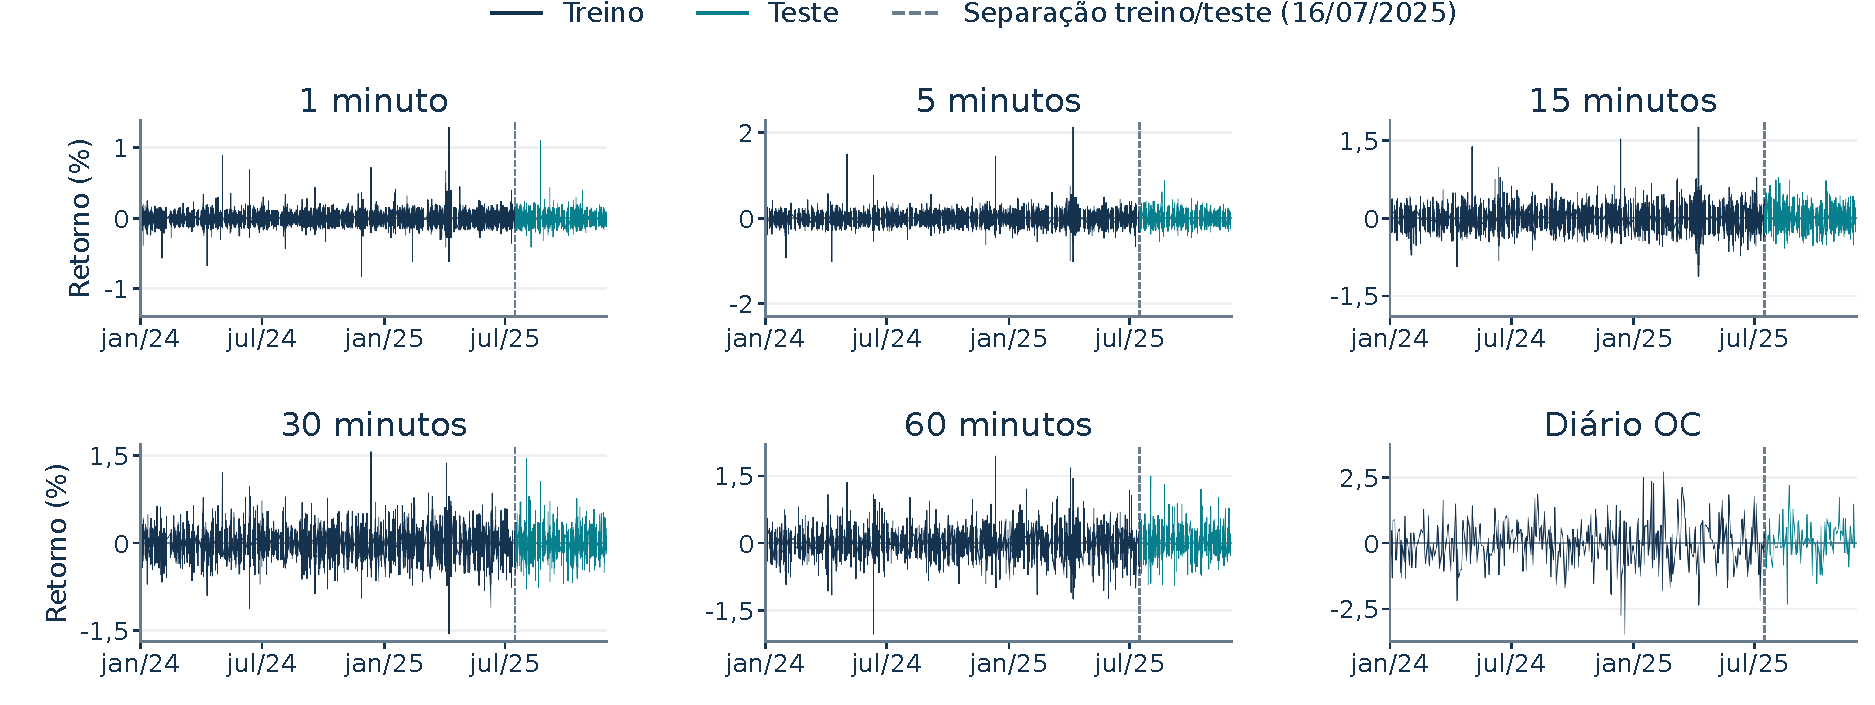
\includegraphics[width=0.98\textwidth,height=5.3cm,keepaspectratio]{figures/00_complete_return_series_slide.pdf}\par\smallskip \scriptsize Eixo horizontal: calendário. Eixos verticais próprios por escala. Todos os retornos, sem suavização. Linha tracejada: novo corte treino/teste.
\source{Inspeção visual | Mesmas séries usadas na análise}{https://github.com/avilarenan/EAD6034/blob/main/src/ead6034/series_overview.py}
\end{frame}

\begin{frame}[t]{Da descrição às hipóteses de dependência}
\tagline{Identificação por FAC/FACP na sequência anual de treino}
\centering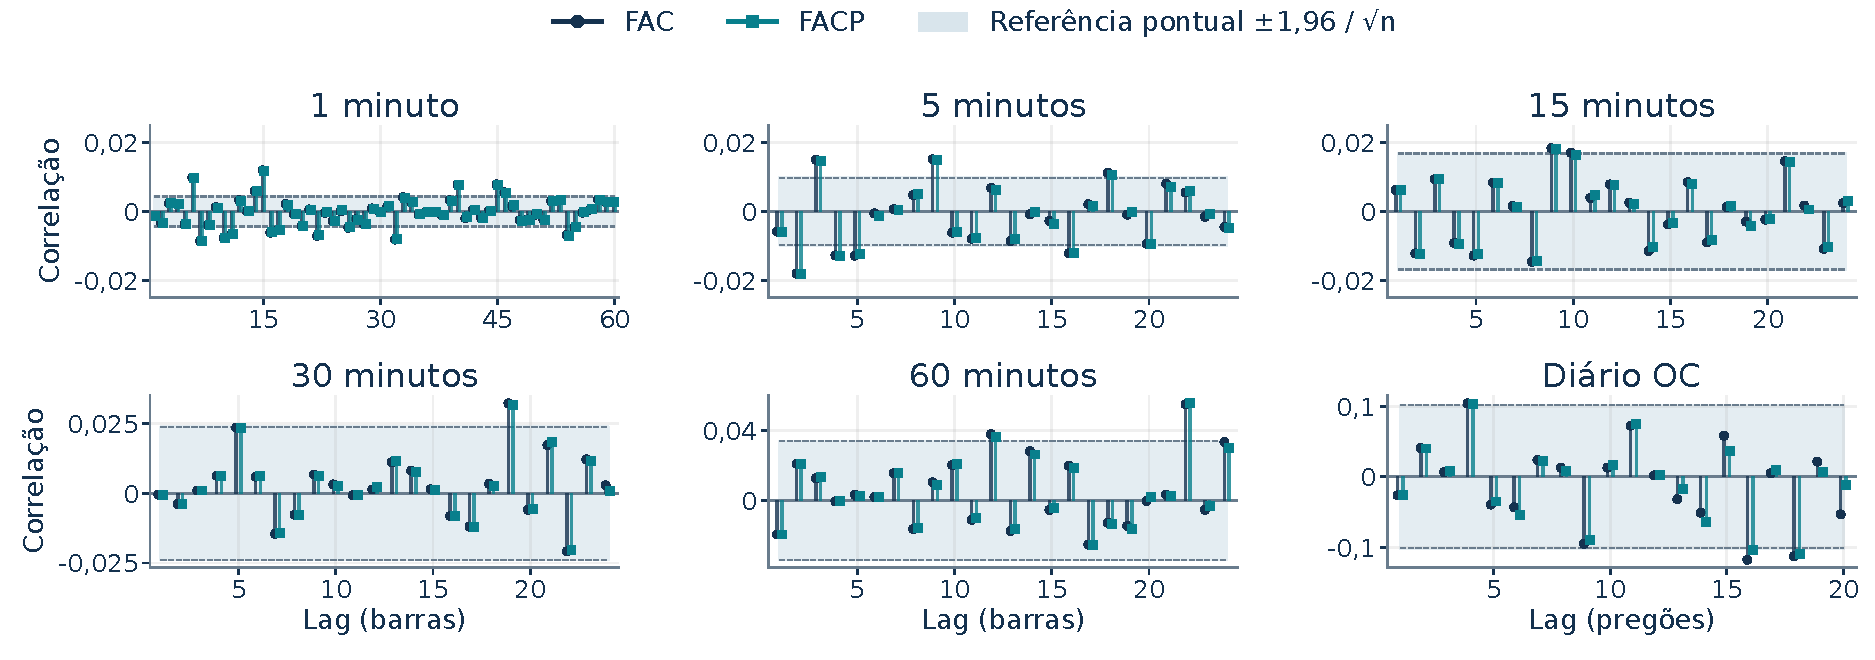
\includegraphics[width=0.98\textwidth,height=5.0cm,keepaspectratio]{figures/01b_return_acf_pacf_slide.pdf}\par\smallskip
\scriptsize Um lag = uma barra da própria escala, inclusive entre pregões. Bandas pontuais sem ajuste para múltiplas comparações.\par Dispersão e dependência na média são propriedades distintas.
\source{Aulas 2--4 | FAC/FACP convencionais}{https://github.com/avilarenan/EAD6034/blob/main/src/ead6034/annual_models.py}
\end{frame}

\begin{frame}[t]{Estacionariedade: três especificações, agora unânimes}
\tagline{ADF (none/drift/trend), PP e KPSS (short/long), 5\% de significância}
\centering\small\begin{tabular}{lrrrrr}
\toprule
Escala & $p$ ADF (3 esp.) & $p$ PP (short/long) & $p$ KPSS-c & $p$ KPSS-ct \\ \midrule
1 min & $<0{,}001$ & $<0{,}001$ / $<0{,}001$ & 0,686 / 0,675 & 0,487 / 0,472 \\
5 min & $<0{,}001$ & $<0{,}001$ / $<0{,}001$ & 0,672 / 0,678 & 0,468 / 0,476 \\
15 min & $<0{,}001$ & $<0{,}001$ / $<0{,}001$ & 0,676 / 0,689 & 0,474 / 0,493 \\
30 min & $<0{,}001$ & $<0{,}001$ / $<0{,}001$ & 0,679 / 0,710 & 0,477 / 0,523 \\
60 min & $<0{,}001$ & $<0{,}001$ / $<0{,}001$ & 0,691 / 0,729 & 0,495 / 0,552 \\
Diário OC & $<0{,}001$ & $<0{,}001$ / $<0{,}001$ & 0,778 / 0,769 & 0,622 / 0,602 \\
\bottomrule
\end{tabular}\par
\raggedright\medskip\small\textbf{ADF e PP:} $H_0$ = raiz unitária. \textbf{Rejeitam em 100\% das 3 especificações $\times$ 6 escalas.}\par\smallskip
\textbf{KPSS} (c e ct, bandas short/long Schwert 1989): \textbf{não rejeita estacionariedade em nenhum caso.}\par
\alert{As três famílias de teste agora concordam} -- sob a divisão anterior (50/50), KPSS-ct rejeitava em todas as escalas; o corte mecânico 80/20 (mais dados de treino) resolveu essa divergência.\par\smallskip
\scriptsize ADF: BIC, até 12 defasagens. PP/KPSS: short $=\lceil4(n/100)^{0{,}25}\rceil$, long $=\lceil12(n/100)^{0{,}25}\rceil$ (convenção do pacote \texttt{arch}, não \texttt{trunc} de \texttt{urca}). Amostra de 1 min: $n=201.960$.
\source{Aula 5 | ur.df/ur.pp/ur.kpss via arch.unitroot}{https://github.com/avilarenan/EAD6034/blob/main/src/ead6034/annual_models.py}
\end{frame}

\begin{frame}[t]{Seleção por BIC e significância dos coeficientes}
\tagline{ARMA(0,0) vence em TODAS as escalas com o novo treino}
\centering\small\setlength{\tabcolsep}{4pt}\begin{tabular}{lcccrc}
\toprule
Escala & ARMA BIC & $\Delta$BIC vs AR(1)/MA(1) & AR(1) $t$ & MA(1) $t$ & Signif. 5\%? \\ \midrule
1 min & (0,0) & 11,87 / 11,87 & $-$0,19 & $-$0,19 & Não \\
5 min & (0,0) & 6,58 / 6,48 & $-$0,59 & $-$0,54 & Não \\
15 min & (0,0) & 8,99 / 8,97 & 0,38 & 0,39 & Não \\
30 min & (0,0) & 8,81 / 8,81 & $-$0,03 & $-$0,03 & Não \\
60 min & (0,0) & 6,86 / 6,91 & $-$0,85 & $-$0,82 & Não \\
Diário OC & (0,0) & 5,67 / 5,69 & $-$0,51 & $-$0,47 & Não \\
\bottomrule
\end{tabular}\par
\raggedright\medskip\small\textbf{Antes} (divisão $\sim$50/50): 1 min selecionava ARMA(2,2), vantagem de só 1,24 de BIC, sem erro-padrão publicado.\par
\textbf{Agora} (80/20, mais treino): \alert{ruído branco vence em todas as escalas}, com folga maior de BIC.\par\smallskip
\scriptsize Erros-padrão: refit com \texttt{cov\_type="robust"} apenas nos $\sim$18 modelos selecionados (não na grade de 216 candidatos). $|t|>1{,}96$ = significativo (Aula 4). O único coeficiente extra de AR(1)/MA(1) nunca é significativo -- reforça, com teste formal, o que o BIC já sugeria.
\source{Aulas 3--4 | Box--Jenkins, alternativas lineares e testes $t$}{https://github.com/avilarenan/EAD6034/blob/main/src/ead6034/annual_models.py}
\end{frame}

\begin{frame}[t]{Volatilidade: GARCH e teste de assimetria (GJR)}
\tagline{Aula 6: constante, ARCH(1), GARCH(1,1) e GJR-GARCH(1,1,1), só no treino}
\centering\small\begin{tabular}{lcrcrc}
\toprule
Escala & Variância BIC & $\alpha+\beta(+\gamma/2)$ & GJR vence? & MSE/const.* & $p$ Q($z^2$) \\ \midrule
1 min & GARCH(1,1) & 0,988 & Não & 1,004 & $<0{,}001$ \\
5 min & GARCH(1,1) & 0,925 & Não & 0,973 & 1,000 \\
15 min & GARCH(1,1) & 0,753 & Não & 0,964 & 0,996 \\
30 min & GARCH(1,1) & 0,557 & Não & 0,989 & $<0{,}001$ \\
60 min & ARCH(1) & 0,146 & Não & 0,981 & $<0{,}001$ \\
Diário OC & Constante & 0,000 & Não & 1,000 & 0,012 \\
\bottomrule
\end{tabular}\par
\raggedright\medskip\small\textbf{GJR-GARCH nunca vence por BIC:} sem evidência de efeito alavancagem (assimetria) nesta série, nestas escalas.\par
\alert{Sem teste Diebold--Mariano entre variâncias:} constante $\subset$ ARCH(1) $\subset$ GARCH(1,1) $\subset$ GJR são aninhados (cada um zera um parâmetro do próximo); a Aula 4 ensina explicitamente que DM não é apropriado para modelos aninhados.\par\smallskip
\scriptsize *MSE da proxy de variância no teste / MSE da variância constante. Estimação sequencial: a previsão pontual do retorno não muda. $\gamma$: 1 min $+$0,0042, 5 min $+$0,0067, 15 min $+$0,0450, 30 min $-$0,0494, 60 min $-$0,0837, diário $+$0,0191 -- pequenos e de sinal instável, consistente com ``nenhum efeito robusto''.
\source{Aula 6 | arch\_model(o=1): GJR-GARCH}{https://github.com/avilarenan/EAD6034/blob/main/src/ead6034/conditional_volatility.py}
\end{frame}

\begin{frame}[t]{A comparação justa usa o mesmo alvo futuro}
\tagline{Parâmetros fixos do treino, somente informação passada em cada origem}
\centering\small\begin{tabular}{lrrrrr}
\toprule
Escala & ARMA & AR & MA & 50/50 & $p$ DM (AR vs MA) \\ \midrule
1 min & 1,0014 & 1,0014 & 1,0014 & 1,0014 & 0,664 \\
5 min & 1,0014 & 1,0007 & 1,0007 & 1,0007 & 0,249 \\
15 min & 1,0014 & 1,0016 & 1,0016 & 1,0016 & 0,413 \\
30 min & 1,0014 & 1,0013 & 1,0013 & 1,0013 & 0,189 \\
60 min & 1,0014 & 0,9999\phantom{9} & 1,0000\phantom{9} & 1,0000\phantom{9} & 0,398 \\
\bottomrule
\end{tabular}\par
\raggedright\medskip\small \textbf{MSE do modelo / MSE do retorno zero: menor que 1 é melhor.} 837 alvos idênticos de 60 minutos, sem sobreposição (93 pregões de teste $\times$ 9 origens).\par
\scriptsize DM compara apenas AR versus MA (não aninhados; ARMA vs AR/MA seria aninhado). Nenhum $p$ rejeita a 5\%. Diferenças de $\sim$0,1\%--0,2\% no MSE, não pontos percentuais de retorno.\par Perdas absolutas e horizonte nativo no relatório completo.
\source{Aula 4 | MSE, combinação e Diebold--Mariano}{https://github.com/avilarenan/EAD6034/blob/main/src/ead6034/forecast_evaluation.py}
\end{frame}

\begin{frame}[t]{Além do currículo: dois baselines exploratórios}
\tagline{Fora da metodologia central (docs/PROTOCOL\_21\_09.md); rotulados como tal}
\begin{columns}[T]\begin{column}{0.5\textwidth}\small
\textbf{MLP} (Aula 4 cita ``ARMA, ETS, MLP, SVM, Deep Learning'' como classes de referência):\par\smallskip
30 defasagens $\to$ 1 retorno futuro. Hiperparâmetros (camada oculta, $\alpha$) escolhidos por MSE de validação = últimos 15\% do treino; \alert{modelo final reajustado em treino+validação} antes do teste -- mesma disciplina do BIC nos modelos lineares.\par\smallskip
MSE/zero (1 min, nativo) $=$ \textbf{1,0051}; $p$ DM vs zero $=$ 0,10 (não significativo).
\end{column}\begin{column}{0.5\textwidth}\small
\textbf{Chronos-2} (``Deep Learning'', zero-shot, sem ajuste algum -- logo sem risco de vazamento por validação):\par\smallskip
Rodado apenas nas 837 origens comuns de 60 min (não em cada minuto: orçamento de CPU), contexto de 512 retornos passados.\par\smallskip
MSE/zero (60 min comum) $=$ \textbf{1,126}; $p$ DM vs zero $=$ \textbf{0,003} (\alert{significativamente pior} que zero).
\end{column}\end{columns}\par\medskip
\scriptsize Nem MLP nem Chronos entram na conclusão central: são um adendo rotulado, não uma reestimação da metodologia aprovada. O resultado de Chronos ilustra que pré-treino genérico não garante desempenho num ativo/frequência específicos sem adaptação.
\source{golden\_rules.md \#1 | Extensão rotulada, não parte da entrega principal}{https://github.com/avilarenan/EAD6034/blob/main/src/ead6034/neural_baselines.py}
\end{frame}

\begin{frame}[t]{Conclusão: alcance dos resultados e da metodologia}
\tagline{Divisão 80/20 corrigida: resultado mais limpo, não apenas conformidade}
\small\textbf{Evidência:} ARMA no alvo comum tem $\sim$0,14\%--0,16\% mais MSE que zero na maioria das escalas; nenhuma diferença é estatisticamente significativa (DM).\par\medskip\begin{columns}[T]\begin{column}{0.50\textwidth}\small\textbf{ARMA de 60 min no teste}\par\smallskip\begin{tabular}{lrr}
\toprule
Recorte & $n$ & MSE/zero \\ \midrule
Início & 93 & 1,0002 \\
Meio & 651 & 1,0015 \\
Fim & 93 & 1,0087 \\
Gap alto & 306 & 1,0008 \\
Gap baixo & 504 & 1,0018 \\
\bottomrule
\end{tabular}\par
\scriptsize Início: 09:05--10:05; meio: até 17:05; fim: até 18:05. Grupos não são aditivos.\end{column}\begin{column}{0.46\textwidth}\small\textbf{Força:} corte 80/20 fixado por contagem de dias, antes de olhar o teste; mesmos alvos e parâmetros fixos do treino.\par\smallskip \textbf{Limites:} contrato por volume diário e dias completos são seleções retrospectivas.\par\smallskip \alert{GJR não achou assimetria; DM não se aplica entre variâncias aninhadas.}\par\smallskip \scriptsize Overnight fora do alvo, mas lags continuam. Resultado restrito a este ativo, janela e modelos; não prova eficiência de mercado.\end{column}\end{columns}\medskip\scriptsize\href{https://github.com/avilarenan/EAD6034/blob/main/results/entrega_28_09}{Relatório, tabelas e código completos}

\source{Síntese dos resultados | Divisão corrigida, significância testada, assimetria testada}{https://github.com/avilarenan/EAD6034/blob/main/src/ead6034/forecast_pipeline.py}
\end{frame}
\begin{frame}[plain,noframenumbering]
\centering\vspace*{1.0cm}{\fontsize{30}{36}\selectfont\bfseries Obrigado\par}\medskip {\Large\color{teal}Perguntas e discussão\par}\vspace{0.9cm}{\large Renan de Luca Avila\par}\smallskip {\normalsize Econometria de Séries Temporais (EAD6034)\par}\vfill{\normalsize\href{https://github.com/avilarenan/EAD6034/blob/main/src/ead6034/forecast_pipeline.py}{Código da análise no GitHub}\par}\medskip {\small\href{https://github.com/avilarenan/EAD6034/tree/main/results/entrega_28_09}{Slides, roteiro e resultados completos}\par}\smallskip {\small\href{https://alphalab.btgpactual.com/datasets/publication:7a74b3ae-90e0-4393-b1e0-01e61c0bedba}{Dados: BTG Alpha Lab, BTG-ATS-A26}\par}\vspace{0.3cm}
\end{frame}

\end{document}
